\chapter{Primer on Tensors}


%\section{Tensors}

Tensors are mathematical entities that are useful to simplify transformations of vectors. Scalars are quantities with magnitude and no direction information. Vectors are quantities with magnitude and one direction information. Tensors are a generalization of this concept. 

Scalars are a zero rank tensor. Vectors are a one rank tensor. A 2nd rank tensor (also called dyad) is a quantity with magnitude and two direction information. The mathematics of tensors allow some equations to be written compactly. 


Let us use an example to illustrate, the stress tensor. In fact, that
was the first tensor described in physics, and it's where the name
comes from: stress, or tension, in Latin {\it tensus}, and thus
tensor.

\section{Scalars and vectors}

Vectors can be multiplied by scalars to produce new vectors with the same  direction.

\begin{equation}
\v{u} = \lambda \v{v}
\end{equation}

\noindent the vector $\v{u}$ has the same direction as the vector
$\v{v}$. The quantity $\lambda$ simply scales the vector
$\v{v}$, which is why $\lambda$ is called a {\it scalar}. They simply scale a vector field. 


Now suppose we wished to alter both the magnitude and the direction of a given vector. Multiplication by a scalar is no longer sufficient. One thing we can do is the cross product between two vectors 

\begin{equation}
\v{u} =  \v{v}\times\v{w}
\end{equation}

Forming the cross product with another vector is also not sufficient, unless we wish to limit the change in direction to right angles. We must find and use another kind of mathematical entity.


\section{Stress tensor}

The classical example of the use of tensors in physics has to do with
stress in a material object. A stress can be applied to a surface
either in the perpendicular or in the parallel direction to the
surface \figp{fig:tensor1}

\begin{figure}
  \begin{center}
    \resizebox{\textwidth}{!}{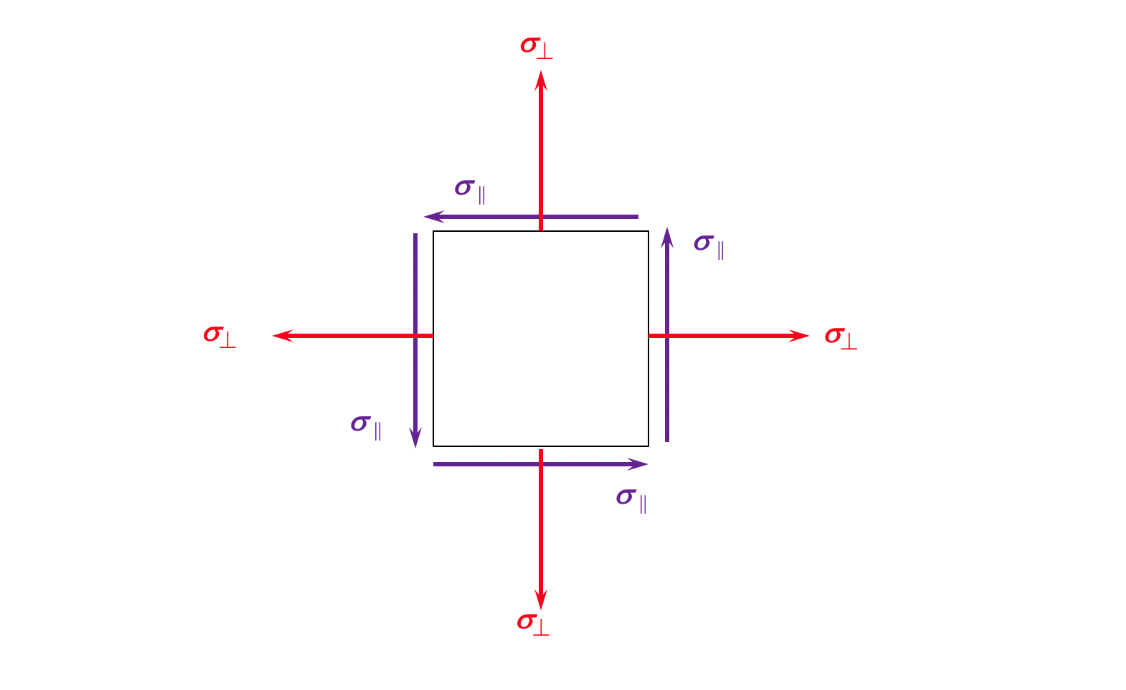
\includegraphics{./figs/TensorsFig01.png}}
  \end{center}
  \caption[]{A stress can be applied to a surface
either in the perpendicular (red arrows) or in the parallel direction
(purple arrows) to the surface.}
  \label{fig:tensor1}
\end{figure}

In the case of the perpendicular direction, the stress leads to
compression or expansion (\fig{fig:tensor2}). The perpendicular stress is a {\it pressure}. 

\begin{figure}
  \begin{center}
    \resizebox{\textwidth}{!}{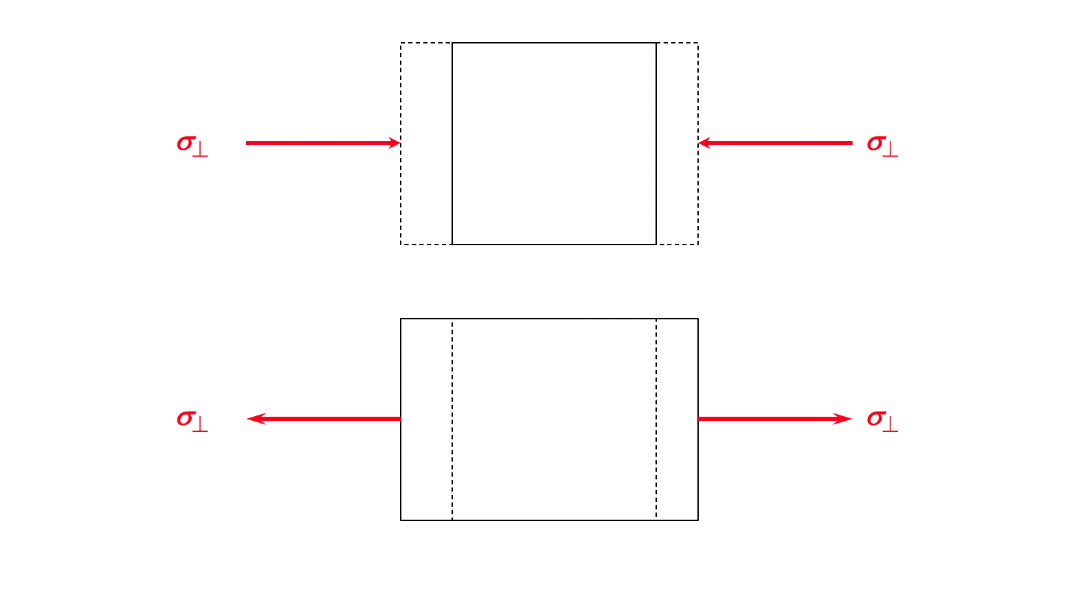
\includegraphics{./figs/TensorsFig02.png}}
  \end{center}
  \caption[]{In the case of the perpendicular direction, the stress leads to
compression or expansion. This is pressure.}
  \label{fig:tensor2}
\end{figure}

In the parallel direction, the surface is transported
(\fig{fig:tensor3}), distorting the
shape in the direction of the applied stress. The parallel stress is a
{\it shear}. 

\begin{figure}
  \begin{center}
    \resizebox{\textwidth}{!}{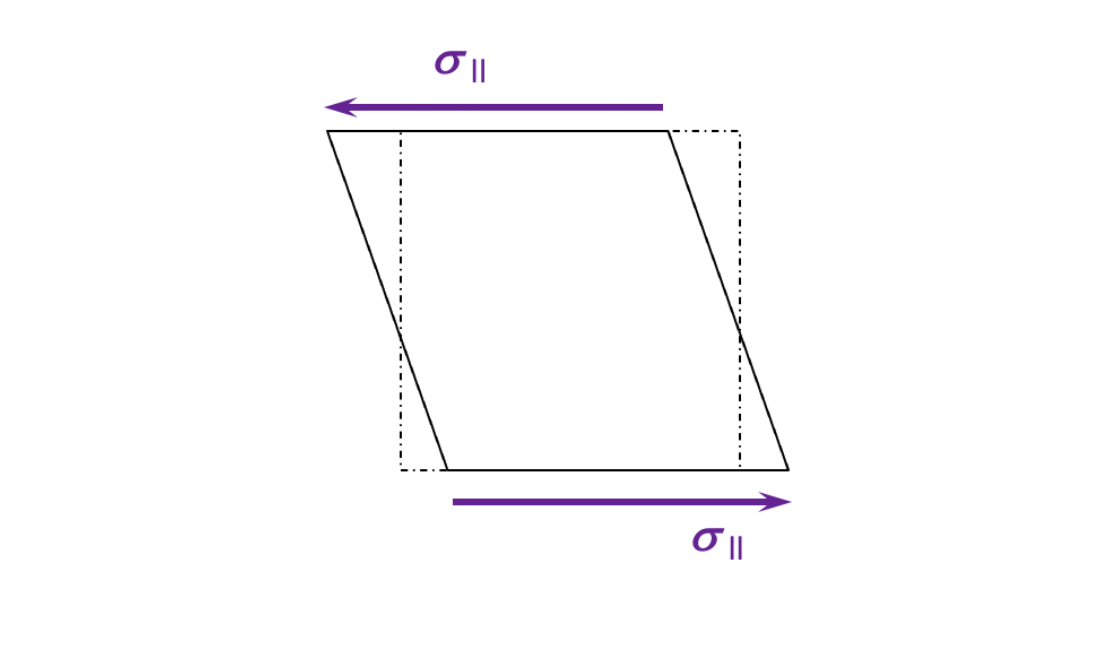
\includegraphics{./figs/TensorsFig03.png}}
  \end{center}
  \caption[]{In the parallel direction, the surface is distorted. The
    parallel stress is a shear.}
  \label{fig:tensor3}
\end{figure}

\section{Mathematizing the stress} 

Stress has units of force per unit area, or dyne/cm$^2$. It seems clear, therefore, that stress $\sigma$ times area $A$ should equal force. In magnitude 

\begin{equation}
F \propto \sigma A 
\end{equation}

\noindent i.e., the stress-area product should be associated with the applied forces that are producing the stress. 


We know that force is a vector. We also know that area can be represented as a vector by associating it with a direction, i.e., the differential area $d\v{A}$ is a vector with magnitude $dA$ and direction normal to the area element $\v{\hat{n}}$.


\begin{equation}
d\v{F} = \vt{\sigma} d\v{A}  
\end{equation}


In this equation, stress can be either a scalar, a vector or something
else. If $\sigma$ were a scalar, then the force would always be in the
direction of the area \fig{fig:tensor4}. This would be fine to describe the pressure, but cannot describe the shear. 

\begin{figure}
  \begin{center}
    \resizebox{\textwidth}{!}{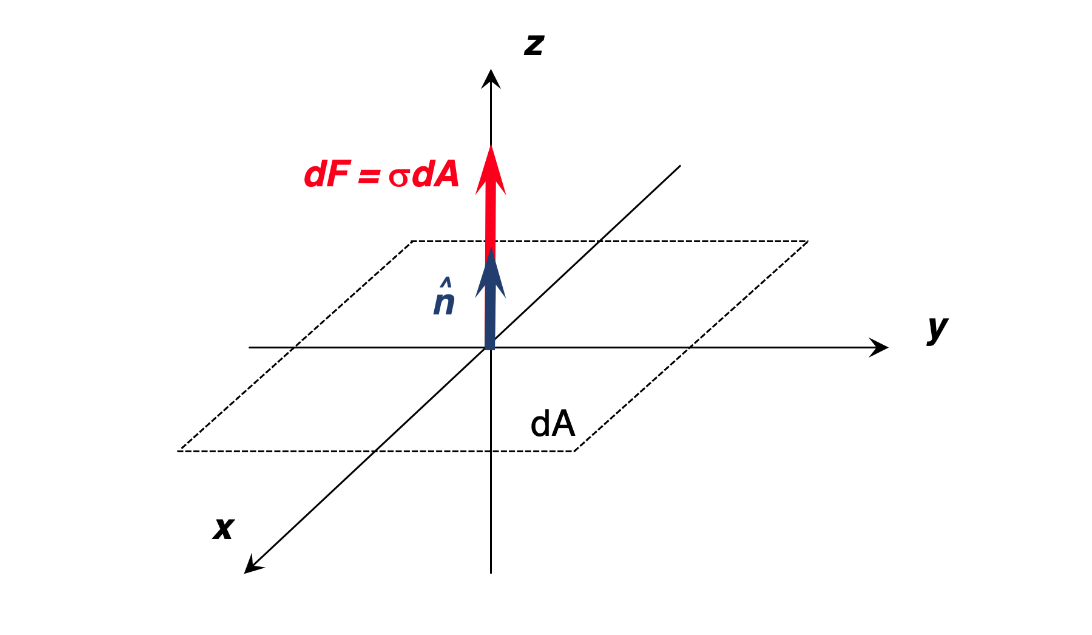
\includegraphics{./figs/TensorsFig04.png}}
  \end{center}
  \caption[]{A scalar stress produces only normal forces.}
  \label{fig:tensor4}
\end{figure}

If, conversely, $\sigma$ were a vector, then to construct a vector out
of the multiplication of two vectors, $\v{\sigma}$ and $d\v{A}$, one would
need a cross product,  $\v{\sigma}\times d\v{A}$. As a consequence,
the force would always be perpendicular to $\v{\sigma}$ and
$d\v{A}$. Perpendicular to $d\v{A}$ means that the force would be in
the plane of the area \fig{fig:tensor5}. While this would be appropriate to describe the shear, it cannot account for the pressure.


\begin{figure}
  \begin{center}
    \resizebox{\textwidth}{!}{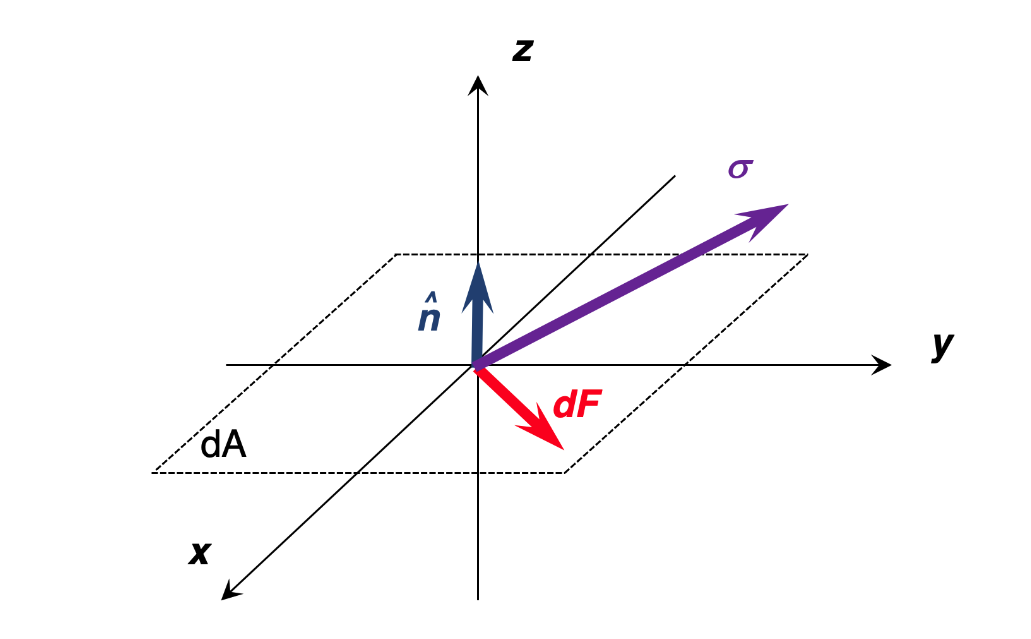
\includegraphics{./figs/TensorsFig05.png}}
  \end{center}
  \caption[]{A vector stress could only produce a shear force.}
  \label{fig:tensor5}
\end{figure}

\section{Toward the tensor formulation}

It seems that {\bf both} scalar and vector stress happen. Operating on
an area, the stress produces a force in all three directions. There
are {\bf pressure} (normal force or tensile stress) and {\bf shear} stress (tangential force). \fig{fig:tensor6} illustrates this. Applied to a surface, the stress produces a force perpendicular to the surface (a pressure), and forces parallel to it (shear). 

\begin{figure}
  \begin{center}
    \resizebox{\textwidth}{!}{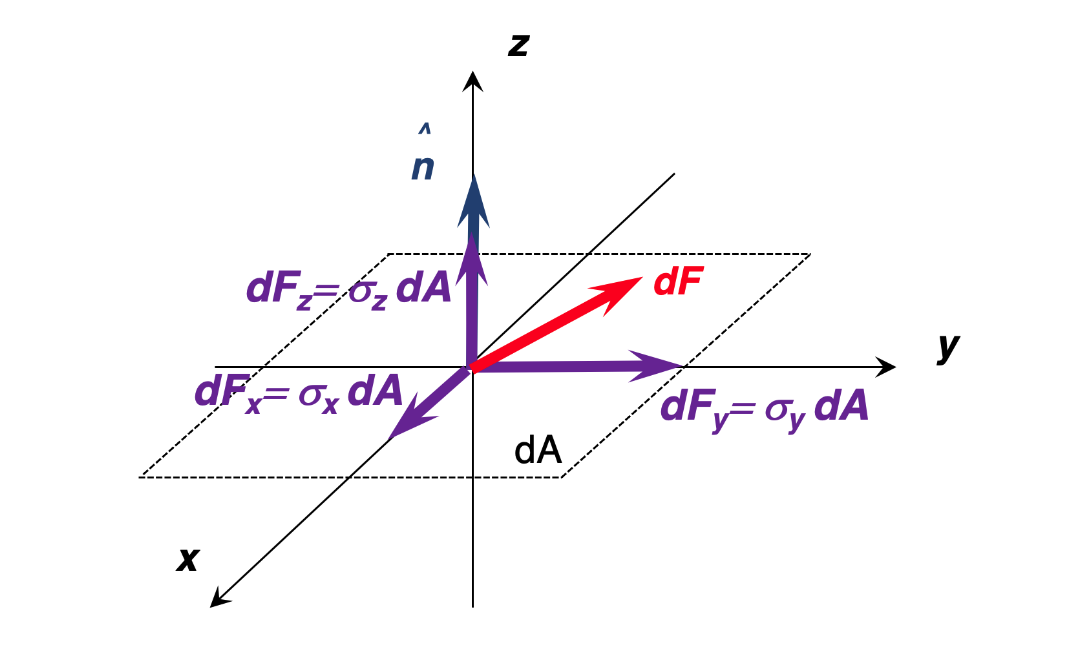
\includegraphics{./figs/TensorsFig06.png}}
  \end{center}
  \caption[]{Applied to a surface, the stress produces a force perpendicular to the surface (a pressure), and forces parallel to it (shear).}
  \label{fig:tensor6}
\end{figure}

\noindent That is, 

\begin{equation}
d\v{F} = \left( \sigma_x \hat{x}+ \sigma_y \hat{y} + \sigma_z\hat{z}  \right) d\v{A}
\label{eq:force-wrong}
\end{equation}

If we want to describe the stress as a single entity, this is neither
a scalar nor a vector. It must be something else that transforms
accordingly to the geometry and algebra above.

\section{Tensor formulation}

The force we found, \eq{eq:force-wrong}, is restricted to the case
where the area is normal to the $z$ direction. Thus, it cannot be the
whole story. Let us consider an area patch in a generic orientation
\figp{fig:tensor7}, where the normal $\v{\hat{n}}=a \v{\hat{x}} + b \v{\hat{y}} + c \v{\hat{z}}$ is a linear combination of the unit Cartesian vectors ($a^2+b^2+c^2=1$). 

\begin{figure}
  \begin{center}
    \resizebox{\textwidth}{!}{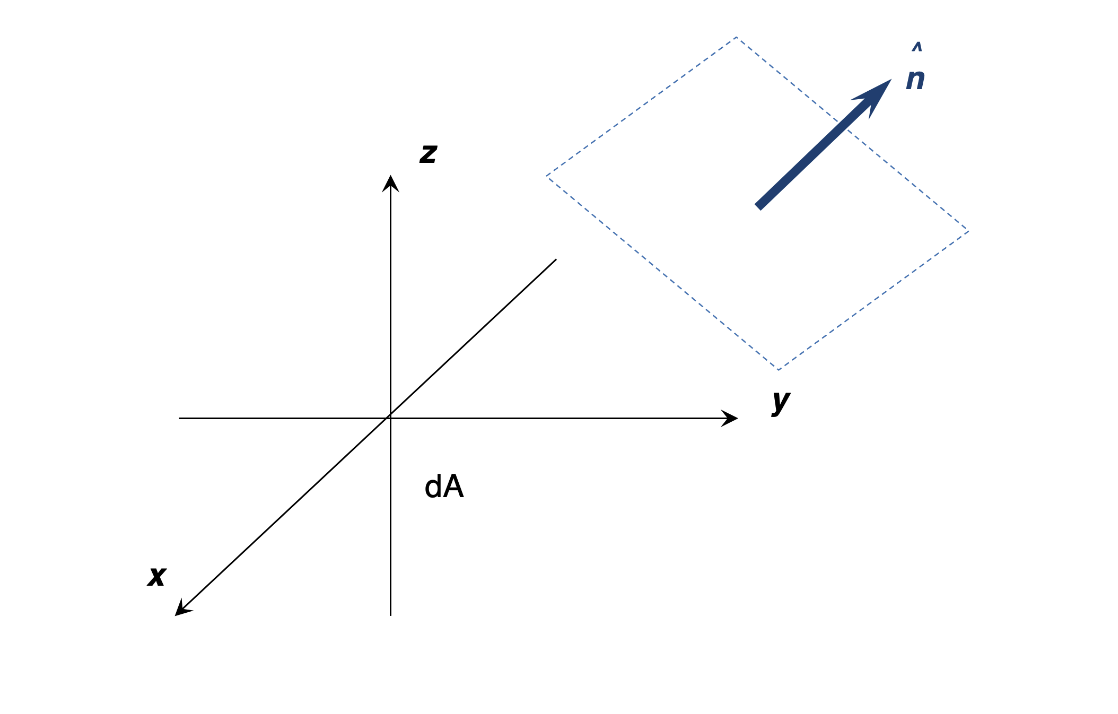
\includegraphics{./figs/TensorsFig07.png}}
  \end{center}
  \caption[]{Area patch in generic orientation.}
  \label{fig:tensor7}
\end{figure}


Let us draw an infinitesimal cube around the origin
\figp{fig:tensor8}. Each surface is normal to the respective unit
vector (what we did before was to consider $z$ only). Each surface will be subject to pressure and shear. So, each surface has a force acting on it, each decomposed in three force components, one in each direction \figp{fig:tensor9}


\begin{figure}
  \begin{center}
    \resizebox{\textwidth}{!}{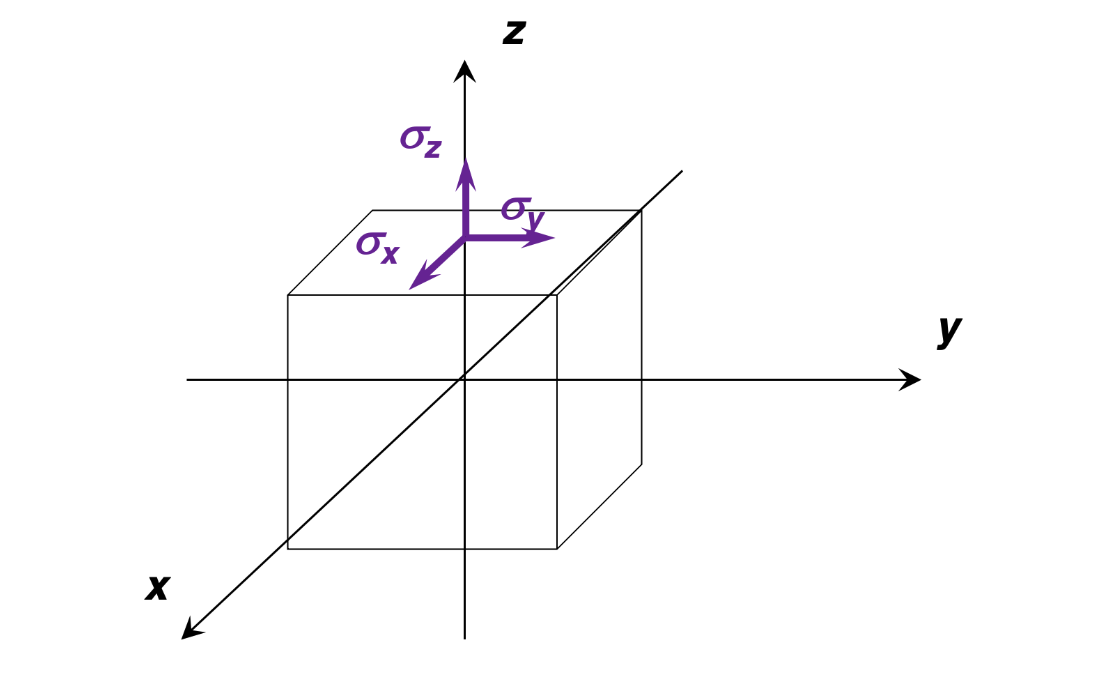
\includegraphics{./figs/TensorsFig08.png}}
  \end{center}
  \caption[]{.}
  \label{fig:tensor8}
\end{figure}


\begin{figure}
  \begin{center}
    \resizebox{\textwidth}{!}{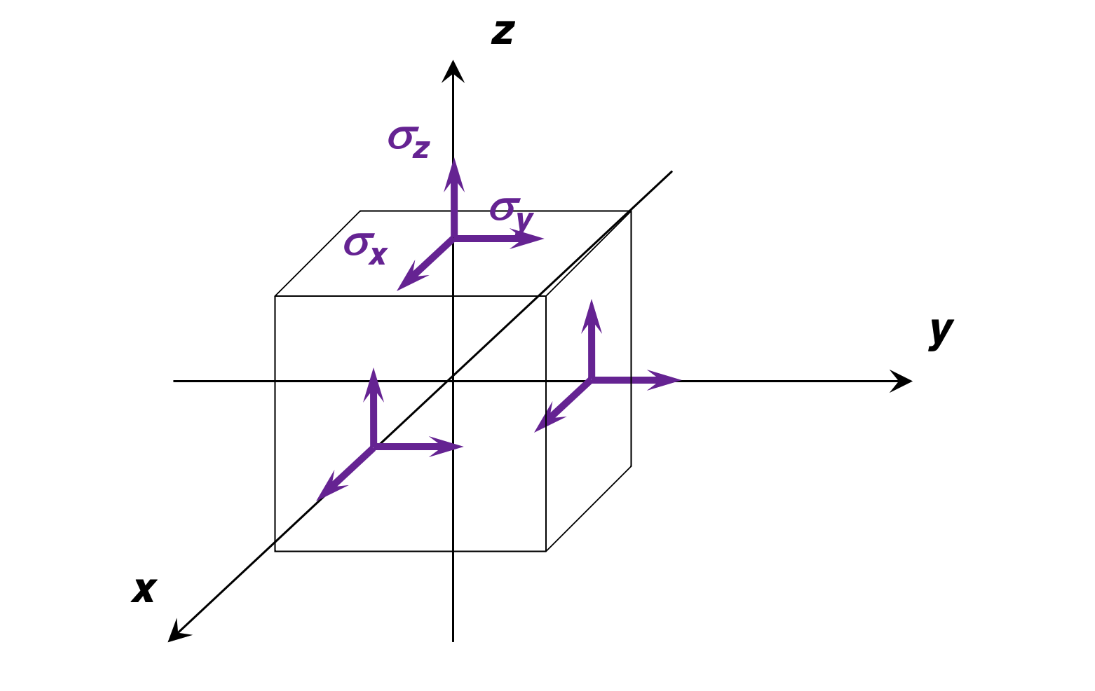
\includegraphics{./figs/TensorsFig09.png}}
  \end{center}
  \caption[]{.}
  \label{fig:tensor9}
\end{figure}

For bookeeping, we give two indices to each stress. The first index
represents the direction, and the second index the surface
\figp{fig:tensor10}. We can now describe the forces acting on each surface \figp{fig:tensor11}.

\begin{figure}
  \begin{center}
    \resizebox{\textwidth}{!}{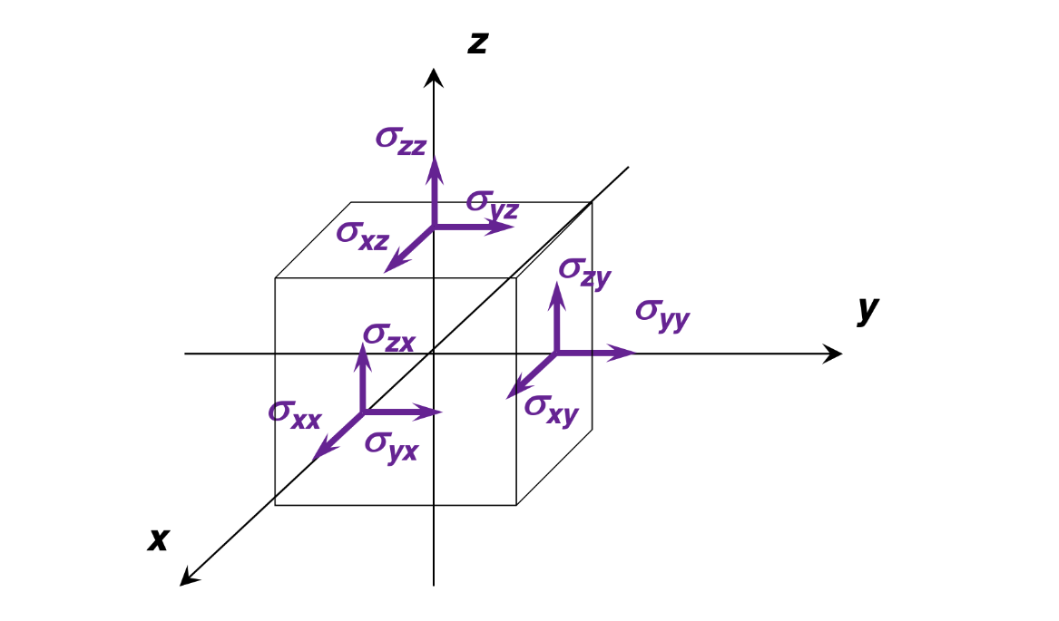
\includegraphics{./figs/TensorsFig10.png}}
  \end{center}
  \caption[]{.}
  \label{fig:tensor10}
\end{figure}

\begin{figure}
  \begin{center}
    \resizebox{\textwidth}{!}{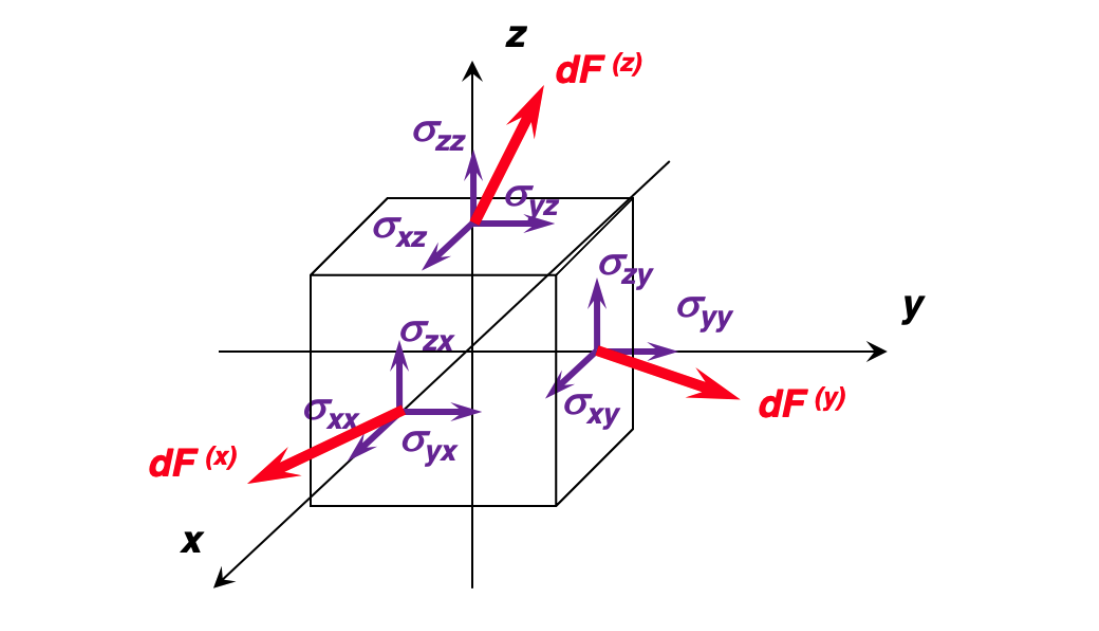
\includegraphics{./figs/TensorsFig11.png}}
  \end{center}
  \caption[]{.}
  \label{fig:tensor11}
\end{figure}

The force in the $x$ surface is 

\begin{equation}
d\v{F}^{(x)} =\left( \sigma_{xx} \hatx + \sigma_{yx} \haty + \sigma_{zx}\hatz  \right) dA_x
\end{equation}

Similarly, the force in the $y$ surface is 


\begin{equation}
d\v{F}^{(y)} =\left( \sigma_{xy} \hatx + \sigma_{yy} \haty + \sigma_{zy}\hatz  \right) dA_y
\end{equation}

and the force in the $z$ surface is 

\begin{equation}
d\v{F}^{(z)} =\left( \sigma_{xz} \hatx + \sigma_{yz} \haty + \sigma_{zz}\hatz  \right) dA_z
\end{equation}



Putting it all together, the force on the cube is  $d\v{F} = d\v{F}^{(x)} + d\v{F}^{(y)} + d\v{F}^{(z)}$, which we can write in components as  

\begin{equation}
d\v{F} = dF_x \hatx + dF_y \haty + dF_z \hatz
\end{equation}

\noindent with 

\begin{eqnarray}
dF_x &=& \sigma_{xx}dA_x + \sigma_{xy}dA_y + \sigma_{xz}dA_z \\
dF_y &=& \sigma_{yx}dA_x + \sigma_{yy}dA_y + \sigma_{yz}dA_z \\
dF_z &=& \sigma_{zx}dA_x + \sigma_{zy}dA_y + \sigma_{zz}dA_z 
\end{eqnarray}

This has the form of a matrix equation  


\begin{equation}
d\v{F} = \vt{\sigma} \cdot d\v{A}
\end{equation}


\noindent so the stress is a {\it matrix}


\begin{equation}
\vt{\sigma} = \left[\begin{array}{ccc}
\sigma_{xx} & \sigma_{xy} & \sigma_{xz} \\
\sigma_{yx} & \sigma_{yy} & \sigma_{yz} \\
\sigma_{zx} & \sigma_{zy} & \sigma_{zz} 
\end{array}\right] 
\end{equation}


\noindent the rows (first index) are the directions, and the columns (second index) are the surfaces. 

Notice that the force is described as the inner product of the stress and the area. This is how matrices behave mathematically: they transform a vector, in both magnitude and direction. 

This is an example of a rank-2 tensor: it needs two directional indices to describe it. Vectors are rank-1 tensors: it needs one directional index to describe them. Scalars are rank-0 tensors: they do not have directional information. 

A vector is a magnitude and direction; it can be expressed as an array once a coordinate system is chosen. Likewise a rank-2 tensor can be expressed as a matrix when a coordinate system is chosen.


\section{Inertia tensor}

Another example is the inertia tensor. Let us consider the angular momentum 

\begin{equation}
\v{L} \equiv m \v{r} \times \v{v}  
\end{equation}


\noindent and the torque that is produced on an object 

\begin{equation}
\v{\tau} \equiv \v{r} \times \v{F}  
\end{equation}

We can specify this relation also in terms of the inertia moment

\begin{equation}
\v{L} \equiv I \v{\omega} 
\end{equation}


which leads to the following equations for rotation kinematics for the relations between torque and angular momentum 


\begin{eqnarray}
\v{\tau} &=& \dot{\v{L}}\\
\v{L} &=&I \v{\omega} 
\end{eqnarray}

which are rotation analogs of the linear relations between force and momentum 

\begin{eqnarray}
\v{F} &=& \dot{\v{p}} \\
\v{p} &=& m \v{v} 
\end{eqnarray}


For forces, $\v{F}=m\v{a}$, since mass is a scalar, the force and acceleration are in the same direction. For rotation, $\v{\tau} = I\v{\alpha}$, a torque produces an angular acceleration $\v{\alpha}\equiv\dot{\v{\omega}}$. 


However, the {\it angular acceleration produced is not necessarily in the same direction as the applied torque}. Depending on the mass distribution, a torque applied in e.g. the $z$ direction can produce rotation around any of the axes.  

A scalar would produce acceleration in the same direction as the
torque, as in force and linear acceleration. Thus, the moment of
inertia is {\it not} a scalar. 

To see how we can cast $\v{\tau}=I\v{\alpha}$ into a form that allows $\v{\tau}$ and $\v{\alpha}$ to be in different directions, let us go back to the definition 

\begin{equation}
\v{L}=m \ \v{r}\times \v{v}
\end{equation}

and write $\v{v} = \v{\omega}\times\v{r}$


\begin{eqnarray}
\v{L} &=& m \ \v{r}\times \v{\omega}\times\v{r}\\
 &=& m \left[r^2\v{\omega} -  \left(\v{r}\cdot \v{\omega}\right)\v{r}\right]\\
\end{eqnarray}


Breaking this into components,  

\begin{eqnarray}
L_x &=& m \left[r^2\omega_x -  \left(x\omega_x + y\omega_y + z\omega_z\right)x\right]\\
L_y &=& m \left[r^2\omega_y -  \left(x\omega_x + y\omega_y + z\omega_z\right)y\right]\\
L_z &=& m \left[r^2\omega_z -  \left(x\omega_x + y\omega_y + z\omega_z\right)z\right]
\end{eqnarray}


and distributing the coordinate  

\begin{eqnarray}
L_x &=& m \left[\left(r^2-x^2\right)\omega_x -  xy\omega_y - xz\omega_z\right]\\
L_y &=& m \left[\left(r^2-y^2\right)\omega_y -  xy\omega_x - yz\omega_z\right]\\
L_z &=& m \left[\left(r^2-z^2\right)\omega_z -  xz\omega_x - yz\omega_y\right]
\end{eqnarray}


writing this in matrix form

\begin{equation}
\v{L}= \vt{I} \cdot \v{\omega}
\end{equation}


where $\vt{I}$ is the following matrix

\begin{equation}
\v{I} = m\left[\begin{array}{ccc}
 \left(r^2-x^2\right) &-  xy &- xz \\
 -  xy & \left(r^2-y^2\right) & - yz \\
 -  xz &- yz & \left(r^2-z^2\right)
\end{array}\right]
\end{equation}


The matrix above is another example of a tensor, the {\bf inertia tensor}. In index notation 

\begin{equation}
I_{ij} = m (r^2 \delta_{ij} - x_ix_j)
\end{equation}


The relationship between torque and angular acceleration is thus 

\begin{equation}
\v{\tau} = \vt{I}\cdot\v{\alpha}
\end{equation}


In full form 

\begin{equation}
\left[\begin{array}{c}
\tau_x\\
\tau_y\\
\tau_z
\end{array}\right] = \left[\begin{array}{ccc}
I_{xx} & I_{xy} & I_{xz} \\
I_{yx} & I_{yy} & I_{yz} \\
I_{zx} & I_{zy} & I_{zz}
\end{array}\right] 
\left[\begin{array}{c}
\alpha_x\\
\alpha_y\\
\alpha_z
\end{array}\right] 
\end{equation}

These are three equations 

\begin{eqnarray}
\tau_x &=& I_{xx}\alpha_x + I_{xy}\alpha_y + I_{xz}\alpha_z\\
\tau_y &=& I_{yx}\alpha_x + I_{yy}\alpha_y + I_{yz}\alpha_z\\
\tau_z &=& I_{zx}\alpha_x + I_{zy}\alpha_y + I_{zz}\alpha_z
\end{eqnarray}


\subsection{Inertia tensor: examples}

Consider a mass $m=1$ in the position (0,1,0). 


\begin{figure}
  \begin{center}
    \resizebox{\textwidth}{!}{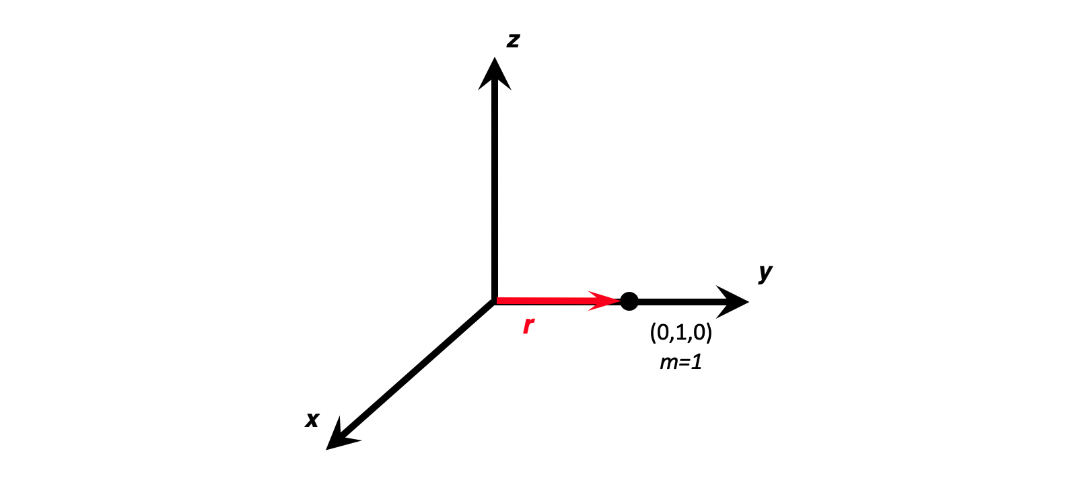
\includegraphics{./figs/TensorsFig12.png}}
  \end{center}
  \caption[]{.}
  \label{fig:tensor12}
\end{figure}


The rotations that the different forces will lead to are: a force in $x$ leads to a rotation around the $z$ axis.  

\begin{figure}
  \begin{center}
    \resizebox{\textwidth}{!}{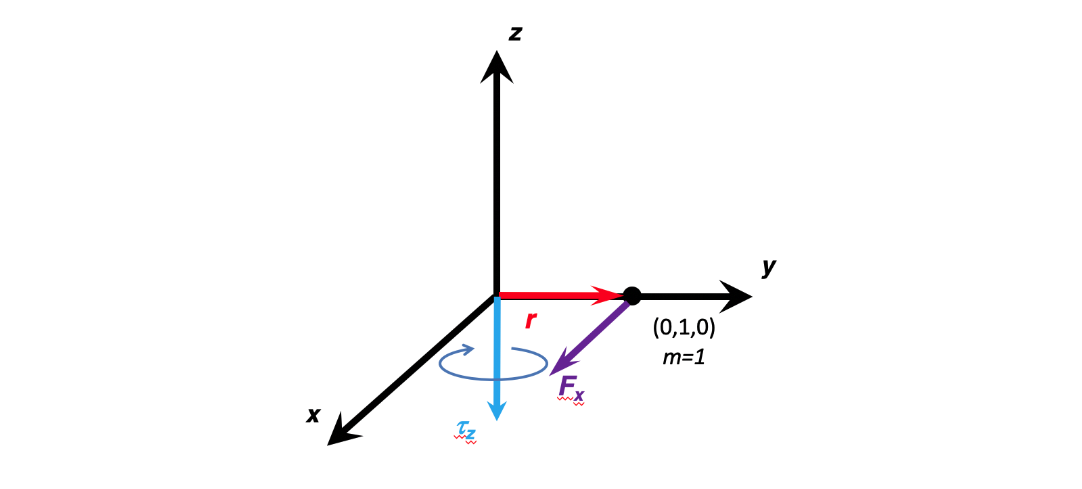
\includegraphics{./figs/TensorsFig13.png}}
  \end{center}
  \caption[]{.}
  \label{fig:tensor13}
\end{figure}

and a force in $z$ leads to a rotation around the $x$ axis. 

\begin{figure}
  \begin{center}
    \resizebox{\textwidth}{!}{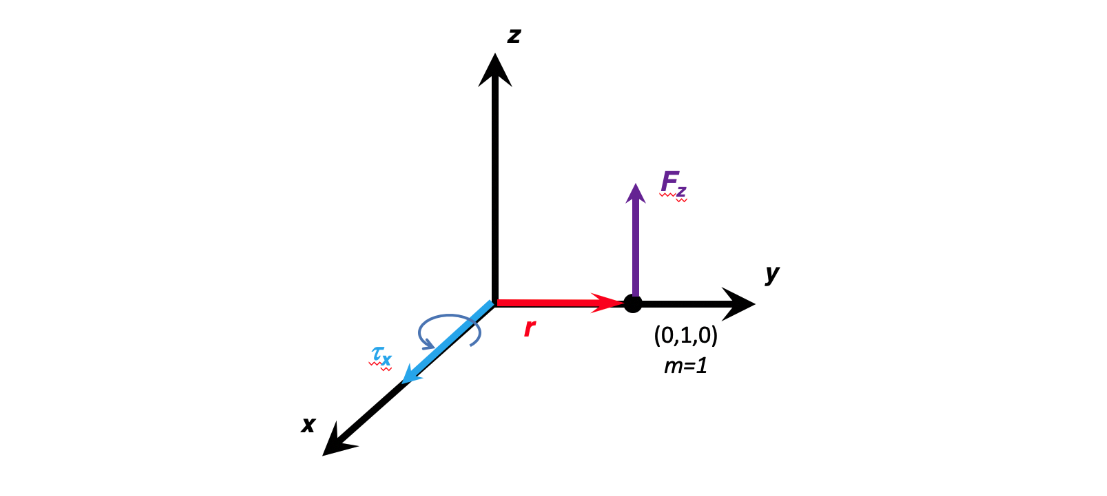
\includegraphics{./figs/TensorsFig14.png}}
  \end{center}
  \caption[]{.}
  \label{fig:tensor14}
\end{figure}

A force in $y$ does not have an arm, so it will not lead to rotation. 

Let us see how the inertia tensor describes this behavior. According to the inertia tensor, the inertia moments are 

\begin{eqnarray}
I_{xx} =I_{zz} &=& 1\\
I_{yy} = I_{xy} = I_{xz} = I_{yz} &=& 0 
\end{eqnarray}

The inertia tensor is thus 
\begin{equation}
I=\left[\begin{array}{ccc}
1 & 0 & 0 \\
0 & 0 & 0 \\
0 & 0 & 1
\end{array}\right] 
\end{equation}

The relationship between torque and acceleration is 


\begin{equation}
\left[\begin{array}{c}
\tau_x\\
\tau_y\\
\tau_z
\end{array}\right] = \left[\begin{array}{ccc}
1 & 0 & 0 \\
0 & 0 & 0 \\
0 & 0 & 1
\end{array}\right] 
\left[\begin{array}{c}
\alpha_x\\
\alpha_y\\
\alpha_z
\end{array}\right] 
\end{equation}

So the torques and accelerations are

\begin{eqnarray}
\tau_x &=& \alpha_x \\
\tau_y &=& 0\\
\tau_z &=& \alpha_z
\end{eqnarray}

The $y$ direction cannot be torqued. The torque in $x$ (a force in the $z$ direction) produces a rotation around the $x$ axis only, as expected. A torque in $z$ (a force in the $x$ direction) produces a rotation around the $z$ axis only, also as expected. 


\subsection{Off-diagonal terms}

Another example. In this case the mass $m=1$ is at $r=(1,1,0)$.

\begin{figure}
  \begin{center}
    \resizebox{\textwidth}{!}{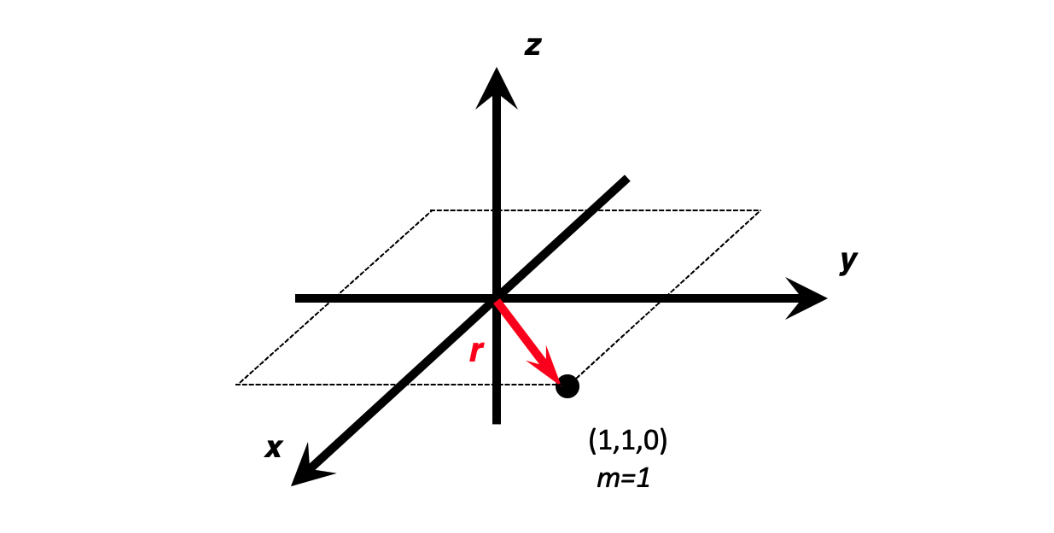
\includegraphics{./figs/TensorsFig15.png}}
  \end{center}
  \caption[]{.}
  \label{fig:tensor15}
\end{figure}

Again, let us understand how the torques will operate. The arm has a component in $x$ and a component in $y$. A force in $x$ will pick the $y$ component of the arm, producing a torque in $z$. 

\begin{figure}
  \begin{center}
    \resizebox{\textwidth}{!}{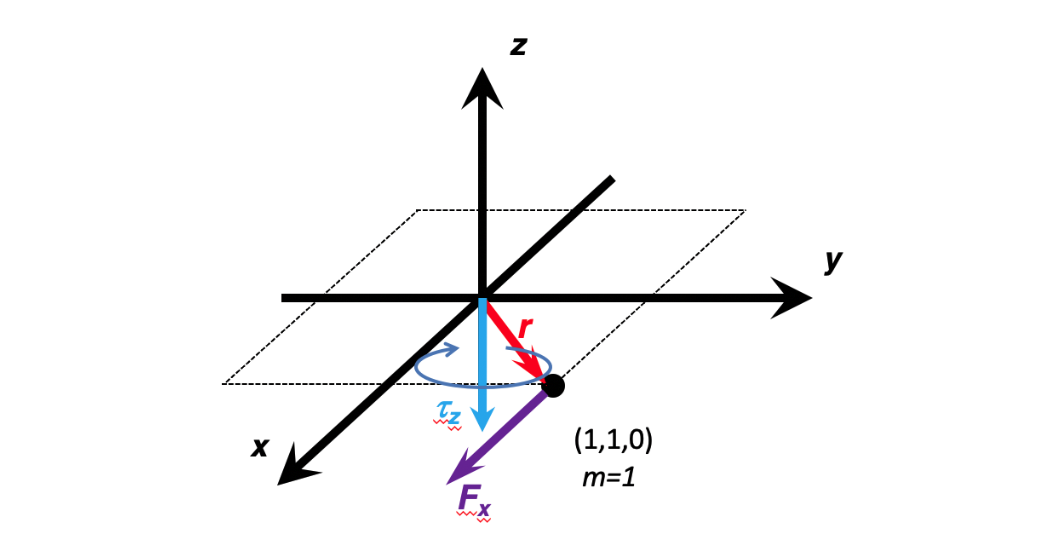
\includegraphics{./figs/TensorsFig16.png}}
  \end{center}
  \caption[]{.}
  \label{fig:tensor16}
\end{figure}

Likewise, a force in $y$ will pick the $x$ component of the arm, also producing a torque in $z$. 

\begin{figure}
  \begin{center}
    \resizebox{\textwidth}{!}{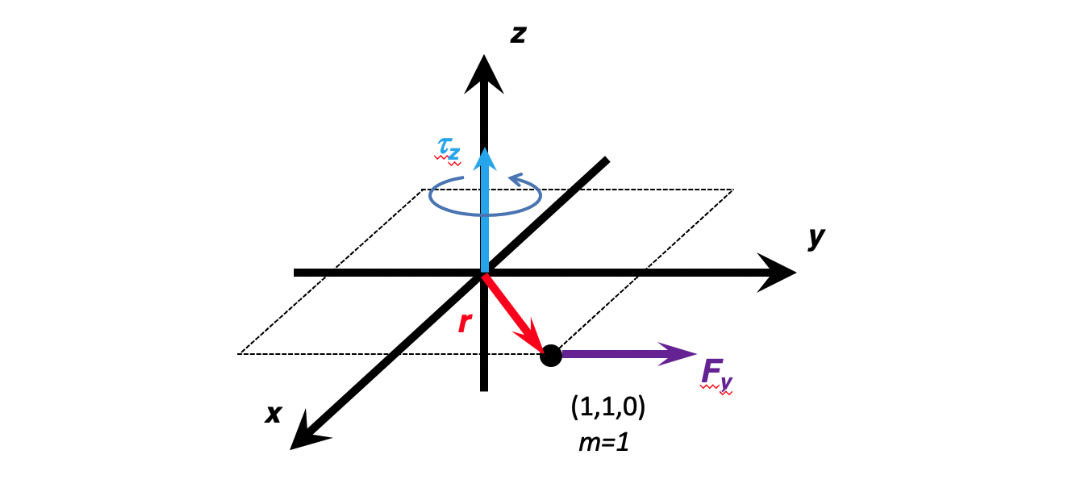
\includegraphics{./figs/TensorsFig17.png}}
  \end{center}
  \caption[]{.}
  \label{fig:tensor17}
\end{figure}

A force in $z$, however, will be picked by both arms, producing torques in both $x$ and $y$. That is to say that if you torque the $x$ direction, a rotation in $y$ will also be produced, and vice versa. 


\begin{figure}
  \begin{center}
    \resizebox{\textwidth}{!}{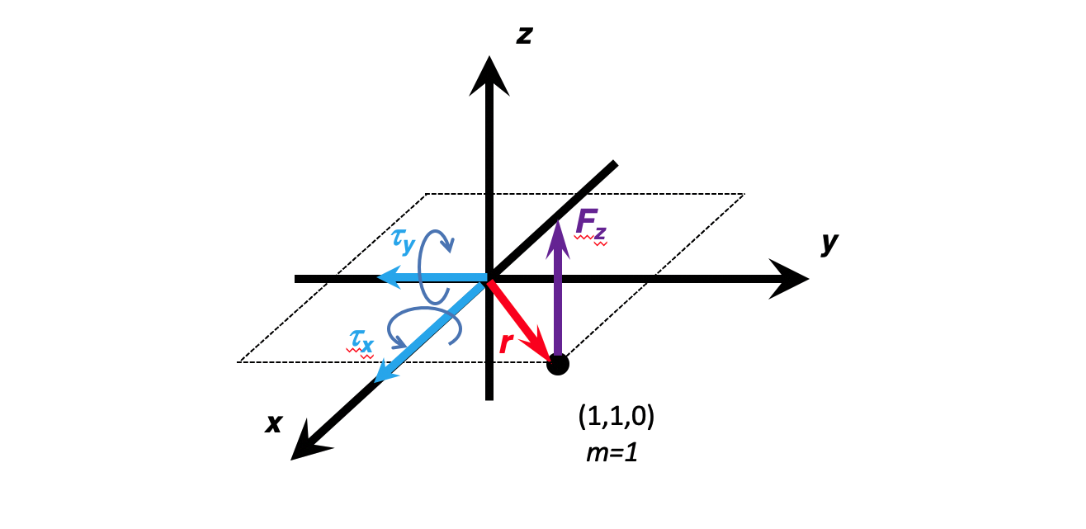
\includegraphics{./figs/TensorsFig18.png}}
  \end{center}
  \caption[]{.}
  \label{fig:tensor18}
\end{figure}


Let us see how the tensor formalism describes this situation.

The inertia moments are

\begin{eqnarray}
I_{xx} = I_{yy} &=& 1\\
I_{zz} &=& 2\\
I_{xy} &=& -1 \\
I_{xz} = I_{yz} &=& 0 
\end{eqnarray}


In matrix form 

\begin{equation}
\left[\begin{array}{c}
\tau_x\\
\tau_y\\
\tau_z
\end{array}\right] = \left[\begin{array}{ccc}
1 & -1 & 0 \\
-1 & 1 & 0 \\
0 & 0 & 2
\end{array}\right] 
\left[\begin{array}{c}
\alpha_x\\
\alpha_y\\
\alpha_z
\end{array}\right] 
\end{equation}

yields these three equations. 

\begin{eqnarray}
\tau_x &=& \alpha_x - \alpha_y  \\
\tau_y &=& -\alpha_x + \alpha_y  \\
\tau_z &=& 2\alpha_z
\end{eqnarray}


Indeed, a torque in $z$ produces a rotation only around the $z$ direction. 

However, a torque in $x$ will not be restricted to the $x$ direction: it will also produce a rotation around the $y$ direction. Moreover, the signs are opposite. A counterclockwise rotation in $x$ will induce a clockwise rotation in $y$. 

Likewise, a torque in $y$ will not be restricted to the $y$ direction either: it will produce a rotation around the $x$ direction as well, of opposite direction. 

This is precisely what we intuitively concluded from examining the
forces with the right-hand-rule. The tensor formalism reaches the same
conclusion, with rigor, and in a more direct way.

A final example, a mass at the position $r=(-1,1,1)$. 

\begin{figure}
  \begin{center}
    \resizebox{\textwidth}{!}{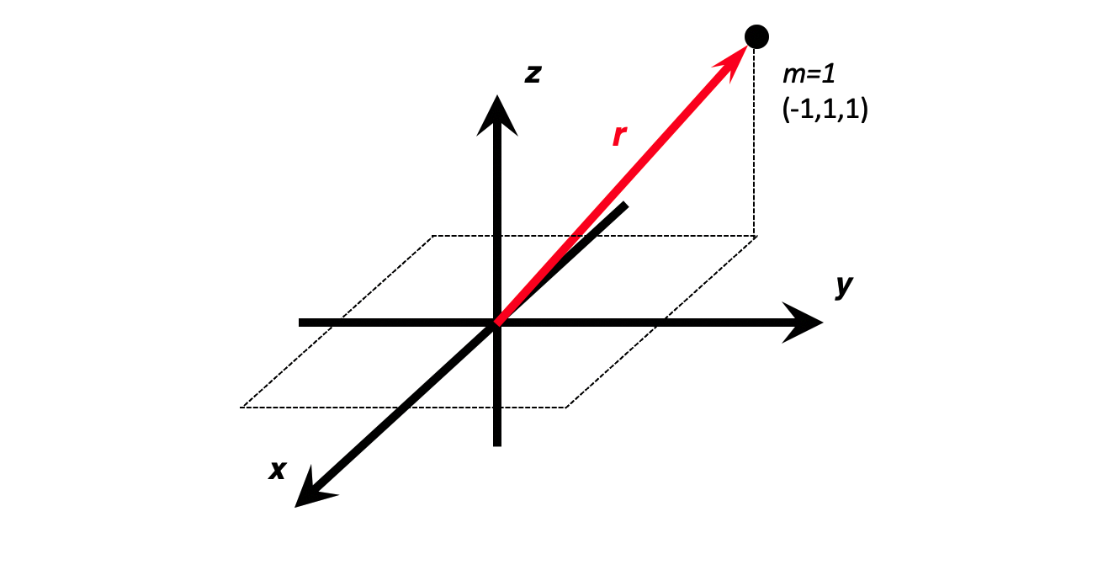
\includegraphics{./figs/TensorsFig19.png}}
  \end{center}
  \caption[]{.}
  \label{fig:tensor19}
\end{figure}

With arms in all direction, we expect that a torque in any direction will produce rotations in all three directions. Let us consider a force in $x$. It will pick the $y$-component of the arm producing a torque in the $z$ direction, and the $z$-component of the arm producing a torque in the $y$ direction.  

\begin{figure}
  \begin{center}
    \resizebox{\textwidth}{!}{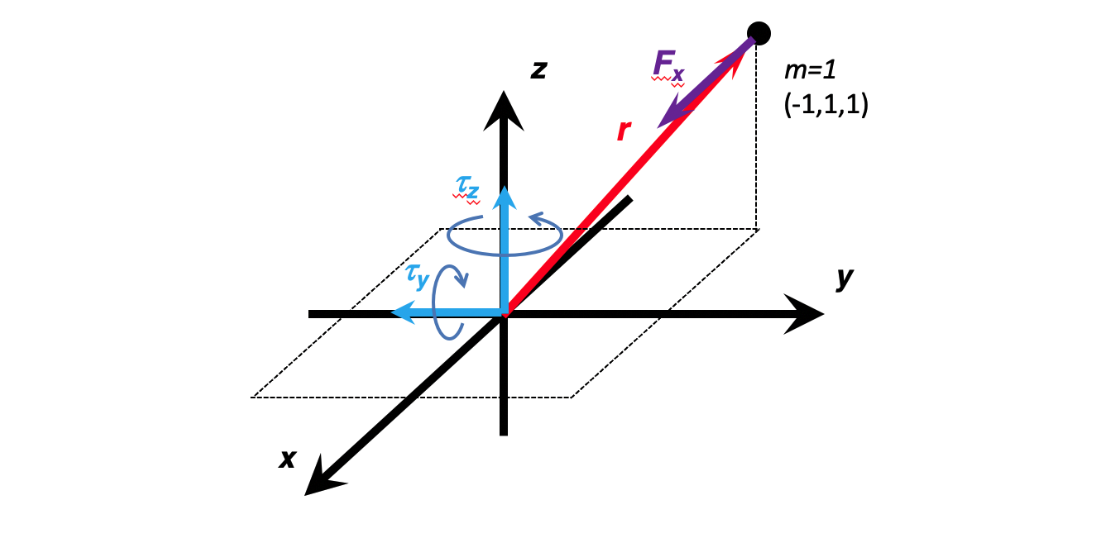
\includegraphics{./figs/TensorsFig20.png}}
  \end{center}
  \caption[]{.}
  \label{fig:tensor20}
\end{figure}


Likewise, a force in $y$ will produce torques in $x$ and $z$. 

\begin{figure}
  \begin{center}
    \resizebox{\textwidth}{!}{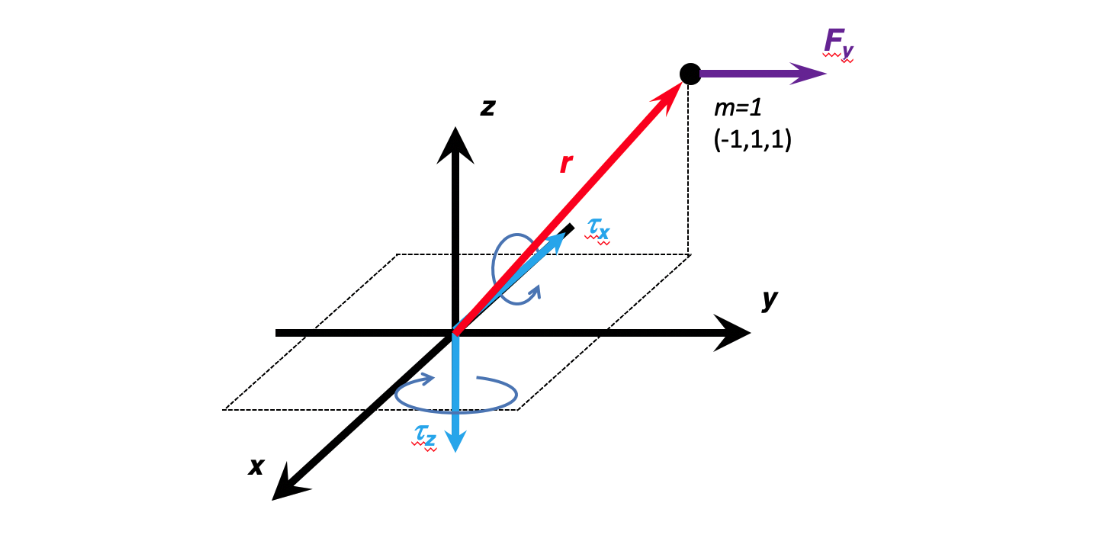
\includegraphics{./figs/TensorsFig21.png}}
  \end{center}
  \caption[]{.}
  \label{fig:tensor21}
\end{figure}


Finally, a force in $z$ will produce torques in $x$ and $y$. 

\begin{figure}
  \begin{center}
    \resizebox{\textwidth}{!}{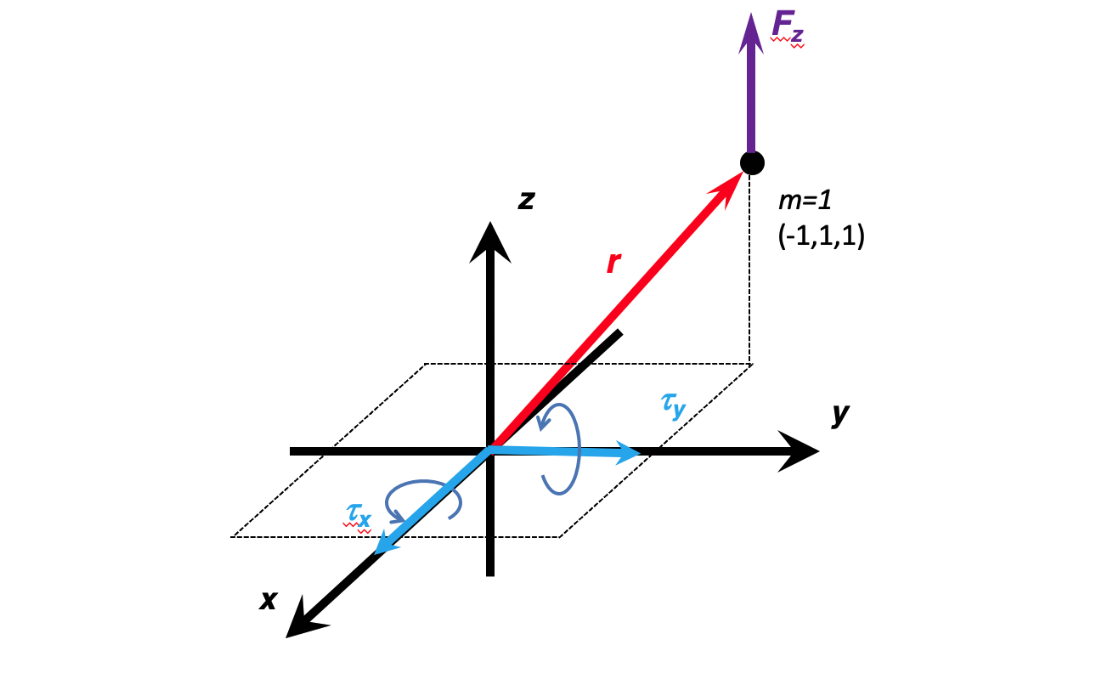
\includegraphics{./figs/TensorsFig22.png}}
  \end{center}
  \caption[]{.}
  \label{fig:tensor22}
\end{figure}


So, indeed, torquing one direction will inevitably produce accelerations in all directions. Let us see how the tensor notation clarifies this behavior. The inertia moments are 

\begin{eqnarray}
I_{xx}=I_{yy}=I_{zz}&=&2\\
I_{xy}=I_{xz}&=&1\\
I_{yz}&=&-1
\end{eqnarray}


So the relationship between torques and angular accelerations is 

\begin{equation}
\left[\begin{array}{c}
\tau_x\\
\tau_y\\
\tau_z
\end{array}\right] = \left[\begin{array}{ccc}
2 & 1 & 1 \\
1 & 2 & -1 \\
1 & -1 & 2
\end{array}\right] 
\left[\begin{array}{c}
\alpha_x\\
\alpha_y\\
\alpha_z
\end{array}\right] 
\end{equation}

These are three equations 

\begin{eqnarray}
\tau_x &=& 2\alpha_x + \alpha_y  + \alpha_z \\
\tau_y &=& \alpha_x + 2\alpha_y  - \alpha_z \\
\tau_z &=& \alpha_x - \alpha_y + 2\alpha_z
\end{eqnarray}


So indeed, a torque in $x$ produces rotation around $x$. The rotation around $x$ induces a rotation around $y$ and around $z$, all in the same sense. 


A torque in $y$ produces a rotation around $y$, which induces a rotation around $x$ and a counter-rotation around $z$.

A torque in $z$ produces a rotation around $z$, which induces a
rotation around $x$ and a counter-rotation around $y$.